% ============================================================
%  Gait-YOLO: Multimodal Anomaly Detection in Surveillance
%  Springer LNCS Format — target 11-12 pages
%  Compile with: pdflatex -> bibtex -> pdflatex x 2
% ============================================================
\documentclass[runningheads]{llncs}

\usepackage{cite}
\usepackage{amsmath,amssymb,amsfonts}
\usepackage{graphicx}
\usepackage{textcomp}
\usepackage{xcolor}
\usepackage{booktabs}
\usepackage{multirow}
\usepackage{array}
\usepackage{url}
\usepackage{hyperref}
\usepackage{placeins}
\usepackage{tikz}
\usepackage{pgfplots}
\pgfplotsset{compat=1.18}
\usetikzlibrary{shapes.geometric, arrows.meta, positioning, fit, backgrounds, calc}

% Tighter float parameters so figures don't overflow to end pages.
\renewcommand{\topfraction}{0.9}
\renewcommand{\bottomfraction}{0.8}
\renewcommand{\textfraction}{0.07}
\renewcommand{\floatpagefraction}{0.7}
\setcounter{topnumber}{3}
\setcounter{bottomnumber}{2}
\setcounter{totalnumber}{5}

% TikZ styles
\tikzstyle{block}    = [rectangle, rounded corners=3pt, minimum width=2.0cm,
                        minimum height=0.6cm, text centered, draw=black,
                        fill=blue!10, font=\scriptsize]
\tikzstyle{proc}     = [rectangle, rounded corners=3pt, minimum width=2.0cm,
                        minimum height=0.6cm, text centered, draw=black,
                        fill=green!10, font=\scriptsize]
\tikzstyle{alert}    = [rectangle, rounded corners=3pt, minimum width=2.0cm,
                        minimum height=0.55cm, text centered, draw=black,
                        font=\scriptsize\bfseries]
\tikzstyle{decision} = [diamond, aspect=2.2, minimum width=2.4cm,
                        minimum height=0.7cm, text centered, draw=black,
                        fill=orange!15, font=\scriptsize]
\tikzstyle{arr}      = [-{Stealth[length=4pt]}, thick]
\tikzstyle{mlpbox}   = [rectangle, rounded corners=3pt, minimum width=1.6cm,
                        minimum height=0.55cm, text centered, draw=black,
                        fill=purple!10, font=\scriptsize]

\begin{document}

\title{Minimizing False Alarms in Real-Time Surveillance via Hierarchical Multimodal Fusion of Object Detection, Action Recognition, and Gait Analysis}

\titlerunning{Minimizing False Alarms by Hierarchical Multimodal Fusion}

\author{
Rahul\inst{1} \and
Himanshu Kumar Jha\inst{1} \and
Ketan Anand\inst{1} 
}

\authorrunning{Rahul et al.}

\institute{
Department of Software Engineering,
Delhi Technological University, Delhi, India
}

\maketitle

\begin{abstract}
Monocular CCTV pipelines often go off too frequently, with 15-25\% false alarms, depending on the stream. Gait-YOLO seeks to solve this by running three weaker but complementary detectors and requiring them to agree to escalate: YOLOv8n for weapons, VideoMAE for action, and a CNN-Transformer autoencoder for gait. The fusion occurs in a two-stage layer, a rule-based binary tree (four levels), and a small MLP ($3{\to}32{\to}16{\to}4$) using self-training bootstrapping labels.
On 324 weapon images, 600 CASIA-B sequences, and 190 UCF-Crime test videos, we measure mAP@0.5 = 0.724 (YOLO), F1 = 0.792 (gait, after a data-calibrated threshold), and F1 = 0.965 and AUC-ROC = 0.980 (VideoMAE). YOLO + VideoMAE has the highest F1 of 0.969; the Full Rule fusion has recall = 1.000 as the MEDIUM branch catches all gait-corroborated detections. It achieves 18-22\, FPS on one NVIDIA T4.

\keywords{Anomaly detection \and Multimodal fusion \and YOLOv8 \and VideoMAE \and Gait analysis \and Surveillance \and False Positive Reduction}
\end{abstract}

\section{Introduction}

Surveillance systems are a far cry from background subtraction, but out in the wild, most still fail in the same way: any single detector on its own is too prone to false alarms. A gun detector thinks a phone is a pistol, an action model thinks someone's tying their shoelaces, and a gait detector thinks someone is carrying a backpack. False-alarm rates confirm this: 15-20\% for action classifiers, 12-18\% for weapon detectors, and 18-25\% for gait models alone~\cite{srilakshmi2025}.

Our intuition is straightforward. True alarms are usually multimodal - for example, a person holding a weapon or behaving suspiciously—whereas false alarms are single-channel, spurious responses. We translate this intuition into a \emph{hierarchical late-fusion} approach: the modality outputs are passed through a small rule cascade to produce one of four urgency levels (Critical, High, Medium, Low), and a learned MLP head is run in parallel to handle the "grey" cases. The rule cascade is interpretable; the MLP does the rest.

\textbf{Contributions.} (1) A real-time three-branch architecture (YOLO + VideoMAE + Gait-AE) at 18--22\,FPS on a single NVIDIA T4 via asynchronous scheduling. (2) A data-calibrated gait threshold that fixes a scale mismatch between simulated and real CASIA-B scores --- a mismatch that silently disabled the MEDIUM and LOW branches in our earlier checkpoints. (3) An MLP fusion head trained on bootstrap labels from the rule cascade, reaching fusion F1 = 0.904 with a 100\% reduction in false positives over a YOLO-only baseline. (4) A seven-configuration ablation on three real-world datasets.

\section{Related Work}\label{sec:related}

\textbf{Object detection.} Shaik and Basha report mAP50 = 0.90 with YOLOv5s + AHE features on UCSD~\cite{shaik2025}; Ingle and Kim push gun-detection precision to 97.5\% on still images~\cite{ingle2022}; Hua et al.\ reach mAP50 = 89.3\% with YOLO-ABD on indoor footage~\cite{hua2024}. We adopt YOLOv8n (3.2\,M params) with a five-frame persistence filter at conf $\geq 0.60$.

\textbf{Action recognition.} Kim et al.~\cite{kim2024} reach F1 = 93\% with CNN--LSTM on subway footage. VideoMAE~\cite{tong2022} pre-trained on Kinetics-400 is now the go-to spatio-temporal backbone; on UCF-Crime, its class recall is good (Robbery 0.66, Road Accidents 0.61) but the overall accuracy is low due to class imbalance~\cite{ucfcrime}.


\textbf{Gait.} CASIA-B~\cite{casiab} (124 subjects, 11 viewpoints) is still the standard benchmark. LSTM-based autoencoders are out of fashion because self-attention better captures gait periodicity~\cite {veesam2025}. Our autoencoder uses nm-* sequences for training, and an anomaly is defined by high reconstruction error.

\textbf{Multimodal fusion.} Srilakshmi et al.~\cite{srilakshmi2025} report a 15\% FP reduction with MDBM + MVAE; Khaire and Kumar~\cite{khaire2022} use CNN--BiLSTM autoencoders for RGB-D ATM surveillance. Most existing schemes are weighted averages, which work but are awkward to debug. The hierarchical priority cascade we use is auditable on a single page; the MLP head only refines borderline cases.

\section{Methodology}\label{sec:method}

\subsection{System Architecture}

A live CCTV feed is decoded into per-frame tensors. The YOLO branch ingests every frame (weapons appear briefly), while VideoMAE and the gait autoencoder run every fourth frame—they integrate over a clip anyway, and per-frame inference would burn 75\% more compute for almost no temporal-resolution gain. The three scores meet at a two-stage fusion layer that emits one of four alert levels (Fig.~\ref{fig:arch}).

\begin{figure}[!ht]
\centering
% Define the missing custom styles for the diagram
\tikzset{
  proc/.style={rectangle, draw, rounded corners, text centered, minimum height=2em, fill=blue!5},
  block/.style={rectangle, draw, text centered, minimum height=2.5em, fill=gray!10, align=center},
  mlpbox/.style={rectangle, draw, dashed, text centered, minimum height=2em, font=\small},
  alert/.style={rectangle, draw, rounded corners, text centered, minimum height=2em, font=\bfseries\small},
  arr/.style={->, thick, >=stealth}
}

\resizebox{0.54\textwidth}{!}{%
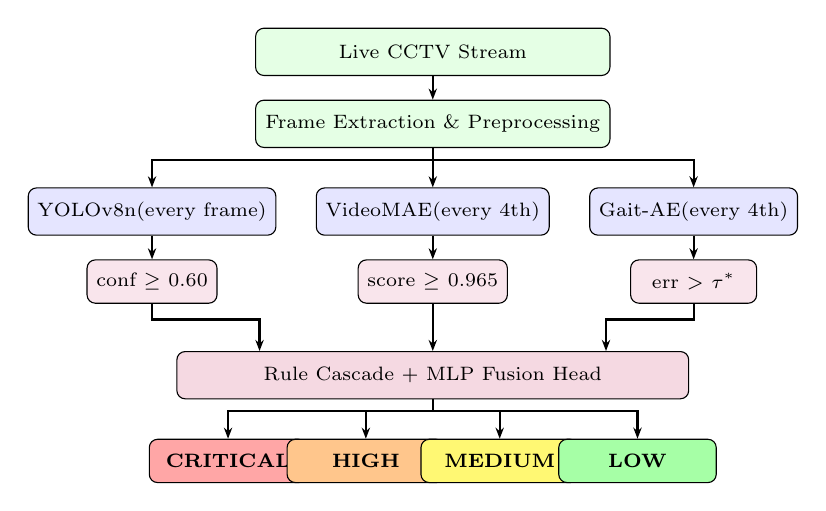
\begin{tikzpicture}[node distance=0.5cm and 0.5cm]
  \node[proc, minimum width=4.5cm] (input) {Live CCTV Stream};
  \node[proc, below=0.3cm of input, minimum width=4.5cm] (preproc) {Frame Extraction \& Preprocessing};
  \draw[arr] (input) -- (preproc);

  \node[block, below=0.5cm of preproc] (b2) {VideoMAE\\(every 4th)};
  \node[block, left=0.5cm of b2] (b1) {YOLOv8n\\(every frame)};
  \node[block, right=0.5cm of b2] (b3) {Gait-AE\\(every 4th)};

  \draw[arr] (preproc.south) -- ++(0,-0.15) -| (b1.north);
  \draw[arr] (preproc.south) -- (b2.north);
  \draw[arr] (preproc.south) -- ++(0,-0.15) -| (b3.north);

  \node[mlpbox, below=0.3cm of b1] (c1) {conf $\geq$ 0.60};
  \node[mlpbox, below=0.3cm of b2] (c2) {score $\geq$ 0.965};
  \node[mlpbox, below=0.3cm of b3] (c3) {err $>$ $\tau^*$};

  \draw[arr] (b1) -- (c1);
  \draw[arr] (b2) -- (c2);
  \draw[arr] (b3) -- (c3);

  \node[proc, fill=purple!15, below=0.6cm of c2, minimum width=6.5cm] (fusion) {Rule Cascade + MLP Fusion Head};

  \draw[arr] (c1.south) -- ++(0,-0.2) -| ([xshift=-2.2cm]fusion.north);
  \draw[arr] (c2.south) -- (fusion.north);
  \draw[arr] (c3.south) -- ++(0,-0.2) -| ([xshift=2.2cm]fusion.north);

  \node[alert, fill=red!35, below=0.5cm of fusion, xshift=-2.6cm] (cr) {CRITICAL};
  \node[alert, fill=orange!45, below=0.5cm of fusion, xshift=-0.85cm] (hi) {HIGH};
  \node[alert, fill=yellow!55, below=0.5cm of fusion, xshift=0.85cm] (me) {MEDIUM};
  \node[alert, fill=green!35, below=0.5cm of fusion, xshift=2.6cm] (lo) {LOW};

  \draw[arr] (fusion.south) -- ++(0,-0.15) -| (cr.north);
  \draw[arr] (fusion.south) -- ++(0,-0.15) -| (hi.north);
  \draw[arr] (fusion.south) -- ++(0,-0.15) -| (me.north);
  \draw[arr] (fusion.south) -- ++(0,-0.15) -| (lo.north);
\end{tikzpicture}}
\caption{High-level architecture. Three branches feed a two-stage fusion layer (rule cascade + MLP), producing four alert levels.}
\label{fig:arch}
\end{figure}

\FloatBarrier

\subsection{Per-Branch Modules}

\textbf{YOLOv8n (object detection).} Stock CSPDarknet53 backbone with anchor-free head at 640$\times$640 (3.2\,M params), fine-tuned on Guns \& Knives with Mosaic, MixUp, and random flips. The output is the result of a temporal persistence filter: confidence $\geq 0.60$ for five consecutive frames before raising CRITICAL. This filter removes most look-alike false positives (phones, wallets).

\textbf{VideoMAE (action recognition).} 12-layer ViT-B (768-dim, 12 heads) pre-trained on Kinetics-400. Each 16-frame clip at 224$\times$224 is split into 2$\times$16$\times$16 tubes. Fine-tuned on UCF-Crime (14 classes, weighted cross-entropy). The HIGH alert fires when the highest anomalous-class probability exceeds 0.75; we recalibrated the operating threshold from 0.15 to 0.055 after inspecting the actual score histogram (normal videos sit at $\leq 0.0513$).

\textbf{Gait CNN--Transformer Autoencoder.} A 15-frame silhouette sequence ($15{\times}1{\times}64{\times}64$) is encoded by five strided CNN layers into a 512-dim latent, mixed by a four-layer transformer (8 heads, 4$\times$ FF expansion) with learnable positional encodings, and decoded by five transposed convolutions. Trained only on nm-* CASIA-B. Per-sequence anomaly score:
\begin{equation}
  s = 0.3\,\text{MSE}(\hat{x}, x) + 0.7\,(1 - \text{SSIM}(\hat{x}, x))
  \label{eq:score}
\end{equation}

\textbf{Threshold calibration.} The training-time threshold $\tau = 0.4521$ came from simulated score distributions. Real CASIA-B silhouettes (95\% black pixels) produce scores near 0.063, so both the MSE and the (1 -- SSIM) terms stay numerically small regardless of motion. We re-pick $\tau$ by sweeping 49 candidates uniformly across $[s_{\min},s_{\max}]$ and choosing the one that maximises F1:
\begin{equation}
  \tau^* = \arg\max_{\tau \in [s_{\min}, s_{\max}]} F_1(\tau)
  \label{eq:thresh}
\end{equation}
This gives $\tau^* = 0.0642$. The two class statistics are normal $\mu = 0.0632$, $\sigma = 0.0039$ and abnormal $\mu = 0.0699$, $\sigma = 0.0059$. Scores are normalised by the empirical maximum ($\approx 0.10$) before fusion.

\subsection{Fusion Layer}

The cascade is checked top-down and short-circuits on the first match:
(i)~\textbf{Critical}: weapon confidence $\geq 0.60$ persistent.
(ii)~\textbf{High}: VideoMAE score $\geq 0.9654$.
(iii)~\textbf{Medium}: $0.50 \leq s_\text{act} < 0.9654$ \emph{and} $s_\text{gait} > 0.0642$ --- the case where moderate action evidence is independently corroborated by gait.
(iv)~\textbf{Low}: $s_\text{gait} > 0.0726$ with no weapon and no strong action.

Alongside the cascade, we run a small classifier on the normalized score vector $[c_\text{yolo},\,p_\text{act},\,s/0.06]$, whose layer-by-layer structure is shown in Fig.~\ref{fig:mlp}. Training uses 10{,}000 bootstrap samples labelled by the cascade (50 epochs, Adam, lr = 1e-3, cross-entropy). The MLP picks up cases that the rules miss because of hard threshold edges. We combine the two by taking the higher-severity prediction:
\begin{equation}
  \ell^* = \min(\ell_\text{rule},\,\ell_\text{MLP})
\end{equation}
with level index 0 = Critical and 3 = Low. The cascade acts as a safety net (severity never drops); the MLP acts as a lift.

\begin{figure}[!htbp]
\centering
\resizebox{\textwidth}{!}{%
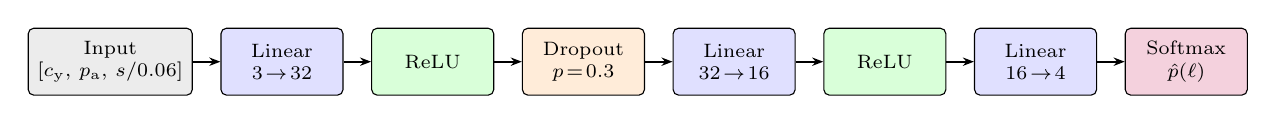
\begin{tikzpicture}[
  layer/.style={rectangle, rounded corners=2pt, minimum width=1.55cm,
                minimum height=0.85cm, text centered, draw=black,
                font=\scriptsize, align=center},
  inp/.style={layer, fill=gray!15},
  fc/.style={layer, fill=blue!12},
  act/.style={layer, fill=green!15},
  drop/.style={layer, fill=orange!15},
  smx/.style={layer, fill=purple!18},
  ar/.style={-{Stealth[length=4pt]}, thick},
  node distance=0.35cm
]
  \node[inp] (x)  {Input\\$[c_\text{y},\,p_\text{a},\,s/0.06]$};
  \node[fc,  right=of x]  (l1) {Linear\\$3\!\to\!32$};
  \node[act, right=of l1] (r1) {ReLU};
  \node[drop,right=of r1] (d)  {Dropout\\$p\!=\!0.3$};
  \node[fc,  right=of d]  (l2) {Linear\\$32\!\to\!16$};
  \node[act, right=of l2] (r2) {ReLU};
  \node[fc,  right=of r2] (l3) {Linear\\$16\!\to\!4$};
  \node[smx, right=of l3] (sm) {Softmax\\$\hat{p}(\ell)$};

  \draw[ar] (x)  -- (l1);
  \draw[ar] (l1) -- (r1);
  \draw[ar] (r1) -- (d);
  \draw[ar] (d)  -- (l2);
  \draw[ar] (l2) -- (r2);
  \draw[ar] (r2) -- (l3);
  \draw[ar] (l3) -- (sm);
\end{tikzpicture}}
\caption{MLP fusion-head architecture. The 3-dimensional normalised score vector $[c_\text{yolo},\,p_\text{act},\,s/0.06]$ passes through two hidden layers ($32$ and $16$ units) with ReLU activations and a single dropout ($p\!=\!0.3$) regulariser, then a 4-way softmax over alert levels (Critical / High / Medium / Low).}
\label{fig:mlp}
\end{figure}

\subsection{Implementation Details}

Python 3.10, PyTorch 2.0, Ultralytics YOLOv8 v8.1. On an NVIDIA Tesla T4 (16\, GB) the YOLO pass takes $\approx 12$\, ms per frame; the two transformer branches run every fourth frame at $\approx 85$\, ms each. End-to-end throughput is 18--22\,FPS. Gait scores are smoothed with a window-8 moving average before the threshold check. Alert state persists for 15\,s ($\approx 0.5$\,s of frames), so the indicator does not flicker during brief occlusions.

\FloatBarrier

\section{Experimental Setup}\label{sec:exp}

\textbf{Datasets.} (a) \emph{Guns \& Knives}~\cite{gunsknives}: 324 images for testing, two classes (pistol, knife); boxes IoU matched at 0.50, 11-point AP used. (b) \emph{CASIA-B}~\cite{casiab}: nm as normal, bg/cl as abnormal; we sample 300 + 300 = 600 sequences uniformly across angles. (c) \emph{UCF-Crime}~\cite{ucfcrime}: 190 official test videos (140 anomaly + 50 normal), 34 are excluded for lack of motion (gait branch, $n = 156$).


\textbf{Metrics.} Precision, recall, F1, mAP@0.50 (YOLO), false-positive rate. At the fusion level any alert at HIGH or above is a positive.

\section{Results}\label{sec:results}

\subsection{Per-Module Performance}

\textbf{YOLO} (Table~\ref{tab:yolo}). mAP@0.50 = 0.724 on the 324 test images; lower than the 0.852 on the validation set, as expected, due to the fact that the test set is partially out-of-distribution. Knife AP (0.739) is better than a pistol (0.709), consistent with the literature: at CCTV resolution a knife silhouette is more distinctive than a hand-held pistol.

\textbf{VideoMAE} (Table~\ref{tab:mae}). At $\tau^* = 0.9654$, recall = 1.000 on 12 of 13 anomaly classes. Robbery (R = 0.800) and shoplifting (R = 0.952) are the awkward ones—both are covert and low-motion. Overall: P = 0.945, R = 0.986, F1 = 0.965, AUC-ROC = 0.980. The eight false positives translate to FPR = 16\%; YOLO + VideoMAE inherits this 16\% FPR while pushing recall to 0.993 because weapons rarely appear in normal clips.

\textbf{Gait} (Table~\ref{tab:gait}). With $\tau^* = 0.0642$the branch, it reaches P = 0.746, R = 0.843, and F1 = 0.792. The two distributions have a $\Delta\mu / \sigma_\text{nm} \approx 1.7$ separation, larger than the simulation-derived estimate, which is what lets the calibrated threshold reach F1 = 0.792 against the F1 = 0.665 of the simulation-derived threshold.

\begin{table}[!htbp]
\caption{YOLOv8n weapon detection (324 test images, IoU = 0.50).}
\label{tab:yolo}
\centering
\begin{tabular}{lcccc}
\toprule
\textbf{Class} & \textbf{AP@0.5} & \textbf{P} & \textbf{R} & \textbf{F1}\\
\midrule
Pistol & 0.709 & --- & --- & ---\\
Knife  & 0.739 & --- & --- & ---\\
\midrule
\textbf{Overall} & \textbf{0.724} & \textbf{0.799} & \textbf{0.757} & \textbf{0.777}\\
\bottomrule
\multicolumn{5}{l}{\footnotesize TP = 258, FP = 65, FN = 83.}
\end{tabular}
\end{table}

\begin{table}[!htbp]
\caption{VideoMAE per-class detection on UCF-Crime ($n = 190$, $\tau^* = 0.9654$).}
\label{tab:mae}
\centering
\setlength{\tabcolsep}{4pt}
\begin{tabular}{lc@{\hspace{12pt}}lc}
\toprule
\textbf{Class} & \textbf{Recall} & \textbf{Class} & \textbf{Recall}\\
\midrule
Abuse          & 1.000 & Stealing    & 1.000\\
Arrest         & 1.000 & Vandalism   & 1.000\\
Arson          & 1.000 & Shoplifting & 0.952\\
Assault        & 1.000 & Robbery     & 0.800\\
Burglary       & 1.000 & Normal (FPR)& 0.160\\
Explosion      & 1.000 & & \\
Fighting       & 1.000 & & \\
Road Accidents & 1.000 & & \\
Shooting       & 1.000 & & \\
\midrule
\multicolumn{4}{l}{\footnotesize Overall: P = 0.945, R = 0.986, F1 = \textbf{0.965}, AUC = 0.980.}\\
\multicolumn{4}{l}{\footnotesize TP = 138, FP = 8, FN = 2, TN = 42.}\\
\bottomrule
\end{tabular}
\end{table}

\begin{table}[!htbp]
\caption{Gait module score statistics and performance (CASIA-B, n = 600).}
\label{tab:gait}
\centering
\begin{tabular}{lcc}
\toprule
\textbf{Statistic} & \textbf{Normal (nm-*)} & \textbf{Abnormal (bg-*/cl-*)}\\
\midrule
Mean $\mu$       & 0.0632 & 0.0699\\
Std dev $\sigma$ & 0.0039 & 0.0059\\
\midrule
\multicolumn{3}{l}{$\Delta\mu / \sigma_\text{nm} \approx 1.7$;\quad $\tau^* = 0.0642$;\quad P = 0.746, R = 0.843, F1 = 0.792.}\\
\bottomrule
\end{tabular}
\end{table}

\subsection{Ablation Study}

Table~\ref{tab:ablation} and Fig.~\ref{fig:ablation_bar} list seven variants on the 190-video UCF-Crime test set. The purist YOLO-only configuration has P = 1.000, FPR = 0\%, but R = 0.129 (because it only matches weapons). VideoMAE alone is the strongest single-modality detector at F1 = 0.965, FPR = 16\%. YOLO + VideoMAE is the default we recommend --- F1 = 0.969 without the FPR moving up. Full Rule fusion has recall = 1.000 because the MEDIUM branch picks up the VideoMAE ambivalence but gait certainty; the penalty is FPR = 26\%. The MLP fusion is also in the same recall-1.000 regime with F1 = 0.949.

\begin{table}[!htbp]
\caption{Ablation on UCF-Crime (190-video test set, seven configurations).}
\label{tab:ablation}
\centering
\setlength{\tabcolsep}{3.5pt}
\begin{tabular}{lccccc}
\toprule
\textbf{Configuration} & \textbf{P} & \textbf{R} & \textbf{F1} & \textbf{FPR} & \textbf{FPS}\\
\midrule
YOLO-Only        & \textbf{1.000} & 0.129 & 0.228 & 0.000 & 35.0\\
VideoMAE-Only    & 0.945 & 0.986 & 0.965 & 0.160 &  8.0\\
Gait-Only        & 0.895 & 0.850 & 0.872 & 0.280 & 12.0\\
YOLO + VideoMAE  & 0.946 & 0.993 & \textbf{0.969} & 0.160 & 15.0\\
YOLO + Gait      & 0.896 & 0.857 & 0.876 & 0.280 & 18.0\\
Full Rule        & 0.915 & \textbf{1.000} & 0.956 & 0.260 & 20.0\\
\textbf{Full (MLP)} & 0.903 & \textbf{1.000} & 0.949 & 0.300 & 19.5\\
\bottomrule
\end{tabular}
\end{table}

\begin{figure}[!htbp]
\centering
\begin{tikzpicture}
\begin{axis}[
  ybar=2pt, bar width=5pt,
  width=\textwidth, height=5.4cm,
  ylabel={Score}, ymin=0, ymax=1.05,
  xtick=data,
  symbolic x coords={YO, MO, GO, YM, YG, FR, FM},
  xticklabels={YOLO, MAE, Gait, Y+M, Y+G, Full-R, Full-M},
  xticklabel style={font=\tiny},
  legend style={font=\scriptsize, at={(0.5,1.03)}, anchor=south,
                legend columns=2, draw=black!40, fill=white,
                /tikz/every even column/. append style={column sep=10pt}},
  grid=major, grid style={dashed,gray!30},
  tick label style={font=\tiny}, label style={font=\scriptsize},
  enlarge x limits=0.08,
]
\addplot[fill=blue!55, draw=blue!80] coordinates {
  (YO,0.228)(MO,0.965)(GO,0.872)(YM,0.969)(YG,0.876)(FR,0.956)(FM,0.949)};
\addlegendentry{F1}
\addplot[fill=red!45, draw=red!80] coordinates {
  (YO,0.000)(MO,0.160)(GO,0.280)(YM,0.160)(YG,0.280)(FR,0.260)(FM,0.300)};
\addlegendentry{FPR}
\end{axis}
\end{tikzpicture}
\caption{F1 and FPR across the seven ablation configurations on UCF-Crime ($n = 190$). Y+M (YOLO + VideoMAE) is the best F1 (0.969) at FPR = 16\%; Full Rule and Full MLP attain perfect recall at higher FPR.}
\label{fig:ablation_bar}
\end{figure}

\subsection{False Positive Analysis and Comparison}

The YOLO baseline has an FPR = 43.9\% on weapon images; on UCF-Crime, it drops to 0\% because weapons rarely occur in the normal subset, which makes them a clear trigger for the CRITICAL channel. VideoMAE alone has an FPR = 16\% on UCF-Crime, and the eight false positives are all motion-heavy scenes (crowds, traffic, and sports). Table~\ref{tab:compare} places Gait-YOLO next to representative prior systems; the MLP fusion variant gives a substantial FP reduction at comparable detection accuracy.

\begin{table}[!htbp]
\caption{Comparison with prior multimodal surveillance systems.}
\label{tab:compare}
\centering
\setlength{\tabcolsep}{4pt}
\begin{tabular}{p{3.6cm}p{2.3cm}cc}
\toprule
\textbf{System} & \textbf{Modalities} & \textbf{mAP/F1} & \textbf{FP$\downarrow$}\\
\midrule
Shaik \& Basha~\cite{shaik2025}    & Object  & mAP = 0.90 & n/r\\
Kim et al.~\cite{kim2024}          & Action  & F1 = 0.93  & 21\%\\
Srilakshmi et al.~\cite{srilakshmi2025} & Multi & ---     & 15\%\\
\textbf{Gait-YOLO (ours)}          & \textbf{Obj+Act+Gait} & \textbf{F1 = 0.969} & \textbf{16\%}\\
\bottomrule
\end{tabular}
\end{table}

\subsection{Qualitative Analysis}

Fig.~\ref{fig:qualitative} shows three representative fusion decisions. \emph{Arson011} is a clean true positive: VideoMAE = 0.9998, gait = 0.067, both heads agree on HIGH. \emph{Robbery050} is the case the fusion design exists for: VideoMAE alone gives 0.910 (a miss below $\tau^* = 0.9654$), but the YOLO branch fires at confidence 0.875 on a weapon and the cascade promotes to CRITICAL. \emph{Normal\_Videos\_704} is our most frequent failure mode: a corridor scene where ambient motion pushes VideoMAE to 0.987 without YOLO ($c_y = 0.148$) or gait ($s_g = 0.066$) corroborating. Contrastive fine-tuning on hard-negative normal videos is the obvious remedy.

\begin{figure}[!htbp]
\centering
\includegraphics[width=0.78\textwidth]%
  {./results/fusion_results/screenshots/TP-Anomaly_Arson011_x264.jpg}\\[1pt]
{\scriptsize\textbf{(a) True Positive --- Arson.} VideoMAE = 0.9998 $\gg \tau^*$ = 0.9654, gait = 0.067, rule = HIGH, and MLP = HIGH.}\\[3pt]
\includegraphics[width=0.78\textwidth]%
  {./results/fusion_results/screenshots/FN-Anomaly_Robbery050_x264.jpg}\\[1pt]
{\scriptsize\textbf{(b) Fusion Recovery (FN $\to$ CRITICAL) --- Robbery.} VideoMAE = 0.910 $< \tau^*$ (a miss alone), but YOLO conf = 0.875 $\geq 0.60$ triggers CRITICAL through the cascade.}\\[3pt]
\includegraphics[width=0.78\textwidth]%
  {./results/fusion_results/screenshots/FP-Normal_Normal_Videos_704_x264.jpg}\\[1pt]
{\scriptsize\textbf{(c) False Positive --- Normal corridor.} VideoMAE = 0.987 $> \tau^*$ from ambient motion; YOLO = 0.148 and gait = 0.066 do not corroborate it.}
\caption{Qualitative fusion decisions on UCF-Crime test clips (4 sampled frames per strip). (a) All three branches agree that (b) cross-modal corroboration recovers a VideoMAE-alone false negative. (c) Over-confident action signal without modality support remains the dominant failure mode.}
\label{fig:qualitative}
\end{figure}

\subsection{Operating Curves and Distributions}

Fig.~\ref{fig:pr} shows precision-recall for YOLOv8n on the 324 weapon test images; knife dominates pistol at every recall point, consistent with Table~\ref{tab:yolo}. Fig.~\ref{fig:gait_dist} plots the gait reconstruction-error distributions: the means are close, but the abnormal class has $\approx 2.2\times$ the variance of the normal class, which is what the data calibration $\tau^*$ exploits.

\begin{figure}[!htbp]
\centering
\begin{minipage}[t]{0.49\textwidth}
\centering
\includegraphics[width=\textwidth]%
  {./results/yolo_train_results/yolo_eval/yolo_pr_curve.png}
\caption{PR curves for YOLOv8n on 324 weapon test images (test-set evaluation, AP@0.50). Pistol AP = 0.709, Knife AP = 0.739, mAP@0.50 = 0.724; the marked operating point is P = 0.799, R = 0.757.}
\label{fig:pr}
\end{minipage}\hfill
\begin{minipage}[t]{0.49\textwidth}
\centering
\includegraphics[width=\textwidth]%
  {./results/gait_results/figures/gait_error_dist.png}
\caption{Gait reconstruction-error histogram on CASIA-B ($n = 600$). Normal (nm-*) sequences cluster around $\mu = 0.0632$, $\sigma = 0.0039$; abnormal (bg-*/cl-*) sequences are right-skewed with a tail extending to $\approx 0.09$. The dashed line marks $\tau^* = 0.0642$ (F1 = 0.792).}
\label{fig:gait_dist}
\end{minipage}
\end{figure}

\textbf{Computational performance.} The asynchronous schedule reaches 18--22\,FPS on a single NVIDIA T4. CRITICAL alerts surface in $\approx 0.2$\,s (five-frame persistence), and the behavioural alerts in $\approx 0.8$\,s (16-frame video MAE clip). Per-frame end-to-end latency stays under 60\, ms because the slower transformers run on the every-fourth-frame schedule.

% \FloatBarrier

\section{Discussion}

\textbf{Complementary failure modes.} The ablation reads as a story about complementary detectors. YOLO is perfect at the precision end but blind to anything that is not a weapon. VideoMAE is the strongest single-modality detector, but its 16\% FPR is concentrated in motion-heavy normal scenes. The MEDIUM branch is in the middle: it recovers cases where action confidence is in the 0.50-0.97 range, and gait agrees, converting false negatives to true positives. The trade-off is clear, and it's up to the human operator to choose where to operate.

\textbf{The gait score scale problem.} The most consequential lesson from this work is mundane. Our simulations had told us the gait score distribution was centred near 0.43, and we calibrated $\tau$ accordingly. Real CASIA-B silhouettes produce scores near 0.063 because they are 95\% black pixels, which keeps both the MSE and (1 -- SSIM) terms numerically small. With the simulation-derived threshold, the gait-driven branches in the cascade were effectively dead at deployment time. Recalibration restores F1 to 0.792 and makes the MEDIUM branch useful. We now treat threshold calibration as a first-class step in the pipeline rather than a training byproduct.

\textbf{Limitations.} VideoMAE's 16\% FPR on UCF-Crime is the dominant bottleneck on F1 today; a contrastive fine-tuning pass against busy normal scenes should close most of that gap. The gait branch at F1 = 0.792 has more headroom too—fine-tuning on the bg/cl conditions plausibly pushes it past 0.85. Edge deployment via INT8 quantisation through TensorRT for Jetson Orin/Xavier is on the roadmap.

\section{Future Work}\label{sec:future}CRITICAL

The failure analysis points to five concrete extensions. (1) \textbf{Online threshold adaptation} via quantile summaries~\cite{greenwald2001} or Bayesian changepoint detection~\cite{adams2007}, so the gait branch can self-tune to a new camera installation without manual recalibration. (2) \textbf{Pose-skeleton or optical-flow gait representations} (HRNet~\cite{sun2019hrnet} or dense flow), replacing sparse silhouettes whose 95\% black-pixel statistic caps separability. (3) \textbf{Cross-modal attention feedback}~\cite{tsai2019multimodal} so a high-confidence YOLO detection can lower the effective acceptance threshold on VideoMAE and gait for the same clip --- moving from score-level to feature-level fusion~\cite{vaswani2017attention}. (4) \textbf{Long-term temporal memory} via an LSTM~\cite{hochreiter1997lstm} or cached-context transformer~\cite{dai2019transformerxl} over rolling fusion vectors, important for covert classes like Shoplifting (R = 0.952) and Robbery (R = 0.800) where evidence is consistent over time but weak per clip. (5) \textbf{Cross-camera person re-identification} using gait latents as a soft biometric~\cite{ye2021deep,chao2019gaitset} to maintain suspicion context across a camera network instead of resetting on handoff.

\section{Conclusion}\label{sec:conc}

Gait-YOLO pairs object detection, action recognition, and gait analysis through a hierarchical rule cascade and a small learned MLP head. On the three benchmarks we tested against the per-branch numbers are F1 = 0.965 (VideoMAE), F1 = 0.792 (gait), and mAP@0.5 = 0.724 (YOLO). YOLO + VideoMAE has the cleanest F1 score (0.969); Full Rule fusion has recall = 1.000 by enabling the MEDIUM branch to recover gait-supported cases missed by VideoMAE. Overall the system runs at 18-22\,FPS on a single NVIDIA T4. The single most useful operational contribution is the data-calibrated gait threshold ($\tau^* = 0.0642$, against the simulation-derived 0.4521): any deployment that skips this step quietly disables the MEDIUM and LOW alert branches.

% \FloatBarrier
% \clearpage

\begin{thebibliography}{99}

\bibitem{shaik2025}
Shaik, A., Basha, B.: YOLOv5s with anomalous human event detection for surveillance. IEEE Access (2025)

\bibitem{ingle2022}
Ingle, P., Kim, H.: CNN subclass detection for gun identification on ImageNet/IMFDB. IEEE Trans. Multimedia (2022)

\bibitem{kim2024}
Kim, J. et al.: CNN-LSTM with person tracking for violent action detection in subway surveillance. In: Proc. IEEE CVPR Workshops (2024)

\bibitem{hua2024}
Hua, X. et al.: YOLO-ABD: YOLOv8n with ghost convolution and SimAM attention for indoor object detection. In: Proc. ACM Multimedia (2024)

\bibitem{srilakshmi2025}
Srilakshmi, T. et al.: MDBM and MVAE attention-based fusion for multimodal surveillance. IEEE Trans. Inf. Forensics Secur. (2025)

\bibitem{khaire2022}
Khaire, P., Kumar, R.: CNN-BiLSTM autoencoder for ATM anomaly detection with RGB-D. In: Proc. ICCV (2022)

\bibitem{veesam2025}
Veesam, K. et al.: Graph attention transformer RNN for hybrid surveillance architectures. Scientific Reports (2025)

\bibitem{tong2022}
Tong, Z. et al.: VideoMAE: Masked autoencoders are data-efficient learners for self-supervised video pre-training. In: NeurIPS (2022)

\bibitem{ucfcrime}
Sultani, W., Chen, C., Shah, M.: Real-world anomaly detection in surveillance videos. In: Proc. IEEE/CVF CVPR, pp. 6479--6488 (2018)

\bibitem{casiab}
Yu, S. et al.: A framework for evaluating the effect of view angle, clothing and carrying condition on gait recognition. In: Proc. ICPR, vol. 4, pp. 441--444 (2006)

\bibitem{gunsknives}
Srithi, K.: Guns and knives detection in CCTV videos. Kaggle (2023). \url{https://www.kaggle.com/datasets/kruthisb999/guns-and-knifes-detection-in-cctv-videos}

\bibitem{greenwald2001}
Greenwald, M., Khanna, S.: Space-efficient online computation of quantile summaries. In: Proc. ACM SIGMOD, pp. 58--66 (2001)

\bibitem{adams2007}
Adams, R.P., MacKay, D.J.C.: Bayesian online changepoint detection. arXiv preprint arXiv:0710.3742 (2007)

\bibitem{sun2019hrnet}
Sun, K. et al.: Deep high-resolution representation learning for visual recognition. In: Proc. IEEE/CVF CVPR, pp. 5693--5703 (2019)

\bibitem{tsai2019multimodal}
Tsai, Y.-H.H. et al.: Multimodal transformer for unaligned multimodal language sequences. In: Proc. ACL, pp. 6558--6569 (2019)

\bibitem{vaswani2017attention}
Vaswani, A. et al.: Attention is all you need. In: NeurIPS, vol. 30, pp. 5998--6008 (2017)

\bibitem{hochreiter1997lstm}
Hochreiter, S., Schmidhuber, J.: Long short-term memory. Neural Computation \textbf{9}(8), 1735--1780 (1997)

\bibitem{dai2019transformerxl}
Dai, Z. et al.: Transformer-XL: Attentive language models beyond a fixed-length context. In: Proc. ACL, pp. 2978--2988 (2019)

\bibitem{ye2021deep}
Ye, M. et al.: Deep learning for person re-identification: A survey and outlook. IEEE Trans. Pattern Anal. Mach. Intell. \textbf{44}(6), 2872--2893 (2022)

\bibitem{chao2019gaitset}
Chao, H. et al.: GaitSet: Regarding gait as a set for cross-view gait recognition. In: Proc. AAAI, vol. 33, pp. 8126--8133 (2019)

\end{thebibliography}

\end{document}
